\documentclass{article}\usepackage[]{graphicx}\usepackage[]{color}
%% maxwidth is the original width if it is less than linewidth
%% otherwise use linewidth (to make sure the graphics do not exceed the margin)
\makeatletter
\def\maxwidth{ %
  \ifdim\Gin@nat@width>\linewidth
    \linewidth
  \else
    \Gin@nat@width
  \fi
}
\makeatother

\definecolor{fgcolor}{rgb}{0.345, 0.345, 0.345}
\newcommand{\hlnum}[1]{\textcolor[rgb]{0.686,0.059,0.569}{#1}}%
\newcommand{\hlstr}[1]{\textcolor[rgb]{0.192,0.494,0.8}{#1}}%
\newcommand{\hlcom}[1]{\textcolor[rgb]{0.678,0.584,0.686}{\textit{#1}}}%
\newcommand{\hlopt}[1]{\textcolor[rgb]{0,0,0}{#1}}%
\newcommand{\hlstd}[1]{\textcolor[rgb]{0.345,0.345,0.345}{#1}}%
\newcommand{\hlkwa}[1]{\textcolor[rgb]{0.161,0.373,0.58}{\textbf{#1}}}%
\newcommand{\hlkwb}[1]{\textcolor[rgb]{0.69,0.353,0.396}{#1}}%
\newcommand{\hlkwc}[1]{\textcolor[rgb]{0.333,0.667,0.333}{#1}}%
\newcommand{\hlkwd}[1]{\textcolor[rgb]{0.737,0.353,0.396}{\textbf{#1}}}%
\let\hlipl\hlkwb

\usepackage{framed}
\makeatletter
\newenvironment{kframe}{%
 \def\at@end@of@kframe{}%
 \ifinner\ifhmode%
  \def\at@end@of@kframe{\end{minipage}}%
  \begin{minipage}{\columnwidth}%
 \fi\fi%
 \def\FrameCommand##1{\hskip\@totalleftmargin \hskip-\fboxsep
 \colorbox{shadecolor}{##1}\hskip-\fboxsep
     % There is no \\@totalrightmargin, so:
     \hskip-\linewidth \hskip-\@totalleftmargin \hskip\columnwidth}%
 \MakeFramed {\advance\hsize-\width
   \@totalleftmargin\z@ \linewidth\hsize
   \@setminipage}}%
 {\par\unskip\endMakeFramed%
 \at@end@of@kframe}
\makeatother

\definecolor{shadecolor}{rgb}{.97, .97, .97}
\definecolor{messagecolor}{rgb}{0, 0, 0}
\definecolor{warningcolor}{rgb}{1, 0, 1}
\definecolor{errorcolor}{rgb}{1, 0, 0}
\newenvironment{knitrout}{}{} % an empty environment to be redefined in TeX

\usepackage{alltt}
\IfFileExists{upquote.sty}{\usepackage{upquote}}{}
\begin{document}

Our GitHub Repository

https://github.com/sabinakou/158francissabina

Our data set:

https://archive.ics.uci.edu/ml/datasets/Automobile

26 variables:

\begin{enumerate}

\item Symboling: the process in which cars are assigned a risk factor associated with price

\item Normalized-losses: continuous from 65 to 256

\item Make: alfa-romeo, audi, bmw, chevrolet, dodge, honda, isuzu, jaguar, mazda, mercedes-benz, mercury, mitsubishi, nissan, peugot, plymouth, porsche, renault, saab, subaru, toyota, volkswagen, volvo, diesel, gas

\item Fuel-type: diesel, gas

\item Aspiration: std, turbo

\item Num-of-doors: four, two 

\item Body-style: hardtop, wagon, sedan, hatchback, convertible

\item Drive-wheels: 4wd, fwd, rwd

\item Engine-location: front, rear

\item Wheel-base: continuous from 86.6 120.9

\item Length: continuous from 141.1 to 208.1

\item Width: continuous from 60.3 to 72.3

\item Height: continuous from 47.8 to 59.8

\item Curb-weight: weight of the car without any people or baggage, continuous from 1488 to 4066

\item Engine-type: dohc, dohcv, l, ohc, ohcf, ohcv, rotor

\item Num-of-cylinders: number of cylinders, eight, five, four, six, three, twelve, two

\item Engine-size: continuous from 61 to 326

\item Fuel-system: types of fuel injections or carburetors, 1bbl, 2bbl, 4bbl, idi, mfi, mpfi, spdi, spfi

\item Bore: the diameter of the cylinder that the piston travels in, continuous from 2.54 to 3.94

\item Stroke: a part of the piston's cycle, continuous from 2.07 to 4.17 

\item Compression-ratio: the ratio of the volume of the cylinder and the combustion chamber when the piston is at the bottom, and the volume of the combustion chamber when the piston is at the top, continuous from 7 to 23

\item Horsepower: continuous from 48 to 288

\item Peak-rpm: peak revolutions per minute, continuous from 4150 to 6600

\item City-mpg: continuous from 13 to 49

\item Highway-mpg: continuous from 16 to 54

\item Price: continuous from 5118 to 45400

\end{enumerate}

The observational units in this data set are the cars. 

\begin{knitrout}
\definecolor{shadecolor}{rgb}{0.969, 0.969, 0.969}\color{fgcolor}\begin{kframe}
\begin{alltt}
\hlstd{imports_85} \hlkwb{<-} \hlkwd{read.csv}\hlstd{(}\hlstr{"https://archive.ics.uci.edu/ml/machine-learning-databases/autos/imports-85.data"}\hlstd{,} \hlkwc{header}\hlstd{=}\hlnum{TRUE}\hlstd{,} \hlkwc{na.strings}\hlstd{=}\hlstr{"?"}\hlstd{)}

\hlkwd{names}\hlstd{(imports_85)} \hlkwb{<-} \hlkwd{c}\hlstd{(}\hlstr{"Symboling"}\hlstd{,} \hlstr{"Normalized-Losses"}\hlstd{,}\hlstr{"Make"}\hlstd{,}\hlstr{"Fuel_Type"}\hlstd{,}\hlstr{"Aspiration"}\hlstd{,}\hlstr{"Num-of-doors"}\hlstd{,}\hlstr{"Body-style"}\hlstd{,}\hlstr{"Drive-wheels"}\hlstd{,}\hlstr{"Engine-location"}\hlstd{,}\hlstr{"Wheel-base"}\hlstd{,}\hlstr{"Length"}\hlstd{,}\hlstr{"Width"}\hlstd{,}\hlstr{"Height"}\hlstd{,}\hlstr{"Curb-weight"}\hlstd{,}\hlstr{"Engine-type"}\hlstd{,}\hlstr{"Num-of-cylinders"}\hlstd{,}\hlstr{"Engine-size"}\hlstd{,}\hlstr{"Fuel-system"}\hlstd{,}\hlstr{"Bore"}\hlstd{,}\hlstr{"Stroke"}\hlstd{,}\hlstr{"Compression-ratio"}\hlstd{,}\hlstr{"Horsepower"}\hlstd{,}\hlstr{"Peak-rpm"}\hlstd{,}\hlstr{"City-mpg"}\hlstd{,} \hlstr{"Highway-mpg"}\hlstd{,}\hlstr{"Price"}\hlstd{)}



\hlkwd{library}\hlstd{(broom)}
\hlkwd{library}\hlstd{(ggplot2)}

\hlkwd{tidy}\hlstd{(imports_85)}
\end{alltt}
\begin{verbatim}
##               column   n         mean           sd   median      trimmed
## 1          Symboling 204 8.235294e-01    1.2390348     1.00 7.987805e-01
## 2  Normalized-Losses 164 1.220000e+02   35.4421675   115.00 1.195076e+02
## 3              Make* 204 1.325490e+01    6.2314731    13.00 1.354268e+01
## 4         Fuel_Type* 204 1.901961e+00    0.2980992     2.00 2.000000e+00
## 5        Aspiration* 204 1.181373e+00    0.3862745     1.00 1.103659e+00
## 6      Num-of-doors* 202 1.435644e+00    0.4970729     1.00 1.419753e+00
## 7        Body-style* 204 3.627451e+00    0.8413169     4.00 3.646341e+00
## 8      Drive-wheels* 204 2.323529e+00    0.5555234     2.00 2.335366e+00
## 9   Engine-location* 204 1.014706e+00    0.1206690     1.00 1.000000e+00
## 10        Wheel-base 204 9.880637e+01    5.9941440    97.00 9.811159e+01
## 11            Length 204 1.740750e+02   12.3621228   173.20 1.738165e+02
## 12             Width 204 6.591667e+01    2.1467163    65.50 6.566524e+01
## 13            Height 204 5.374902e+01    2.4249014    54.10 5.371768e+01
## 14       Curb-weight 204 2.555603e+03  521.9608201  2414.00 2.512835e+03
## 15      Engine-type* 204 4.029412e+00    1.0358679     4.00 4.048780e+00
## 16 Num-of-cylinders* 204 3.117647e+00    0.7977075     3.00 3.060976e+00
## 17       Engine-size 204 1.268922e+02   41.7445685   119.50 1.205244e+02
## 18      Fuel-system* 204 4.245098e+00    2.0144125     6.00 4.304878e+00
## 19              Bore 200 3.329050e+00    0.2740440     3.31 3.325625e+00
## 20            Stroke 200 3.258300e+00    0.3148679     3.29 3.279625e+00
## 21 Compression-ratio 204 1.014814e+01    3.9810001     9.00 9.036707e+00
## 22        Horsepower 202 1.042228e+02   39.8101824    95.00 9.914815e+01
## 23          Peak-rpm 202 5.125990e+03  480.4436796  5200.00 5.127469e+03
## 24          City-mpg 204 2.524020e+01    6.5515126    24.00 2.478049e+01
## 25       Highway-mpg 204 3.076961e+01    6.8983369    30.00 3.042073e+01
## 26             Price 200 1.320569e+04 7966.9825580 10270.00 1.166558e+04
##            mad     min      max   range        skew    kurtosis
## 1     1.482600   -2.00     3.00     5.0  0.21160174 -0.69232152
## 2    35.582400   65.00   256.00   191.0  0.75202161  0.43096650
## 3     8.895600    1.00    22.00    21.0 -0.23927514 -1.20785284
## 4     0.000000    1.00     2.00     1.0 -2.68360594  5.22743750
## 5     0.000000    1.00     2.00     1.0  1.64165941  0.69854181
## 6     0.000000    1.00     2.00     1.0  0.25765977 -1.94315763
## 7     1.482600    1.00     5.00     4.0 -0.59977357  0.87300279
## 8     0.000000    1.00     3.00     2.0 -0.04897452 -0.70247720
## 9     0.000000    1.00     2.00     1.0  8.00396793 62.36930651
## 10    3.854760   86.60   120.90    34.3  1.05346680  0.94135120
## 11   10.304070  141.10   208.10    67.0  0.14766484 -0.14856519
## 12    2.075640   60.30    72.30    12.0  0.88389719  0.61137100
## 13    2.372160   47.80    59.80    12.0  0.07530151 -0.48309122
## 14  575.248800 1488.00  4066.00  2578.0  0.66958403 -0.11392044
## 15    0.000000    1.00     7.00     6.0 -0.48170196  3.29135602
## 16    0.000000    1.00     7.00     6.0  2.10594434 10.59013452
## 17   33.358500   61.00   326.00   265.0  1.91564984  5.03220324
## 18    1.482600    1.00     8.00     7.0 -0.23069873 -1.65931314
## 19    0.385476    2.54     3.94     1.4  0.02667500 -0.86485480
## 20    0.252042    2.07     4.17     2.1 -0.68507216  2.05499893
## 21    0.593040    7.00    23.00    16.0  2.56388953  4.95117083
## 22   37.065000   48.00   288.00   240.0  1.36988333  2.45426481
## 23  444.780000 4150.00  6600.00  2450.0  0.06824582 -0.01726486
## 24    7.413000   13.00    49.00    36.0  0.64629733  0.48910757
## 25    7.413000   16.00    54.00    38.0  0.52479839  0.35435460
## 26 4902.216900 5118.00 45400.00 40282.0  1.77880455  3.03214923
##              se
## 1  8.674979e-02
## 2  2.767568e+00
## 3  4.362904e-01
## 4  2.087112e-02
## 5  2.704462e-02
## 6  3.497392e-02
## 7  5.890397e-02
## 8  3.889441e-02
## 9  8.448517e-03
## 10 4.196740e-01
## 11 8.655217e-01
## 12 1.503002e-01
## 13 1.697771e-01
## 14 3.654457e+01
## 15 7.252526e-02
## 16 5.585070e-02
## 17 2.922704e+00
## 18 1.410371e-01
## 19 1.937784e-02
## 20 2.226453e-02
## 21 2.787258e-01
## 22 2.801035e+00
## 23 3.380390e+01
## 24 4.586976e-01
## 25 4.829802e-01
## 26 5.633507e+02
\end{verbatim}
\begin{alltt}
\hlkwd{tidy}\hlstd{(imports_85)}
\end{alltt}
\begin{verbatim}
##               column   n         mean           sd   median      trimmed
## 1          Symboling 204 8.235294e-01    1.2390348     1.00 7.987805e-01
## 2  Normalized-Losses 164 1.220000e+02   35.4421675   115.00 1.195076e+02
## 3              Make* 204 1.325490e+01    6.2314731    13.00 1.354268e+01
## 4         Fuel_Type* 204 1.901961e+00    0.2980992     2.00 2.000000e+00
## 5        Aspiration* 204 1.181373e+00    0.3862745     1.00 1.103659e+00
## 6      Num-of-doors* 202 1.435644e+00    0.4970729     1.00 1.419753e+00
## 7        Body-style* 204 3.627451e+00    0.8413169     4.00 3.646341e+00
## 8      Drive-wheels* 204 2.323529e+00    0.5555234     2.00 2.335366e+00
## 9   Engine-location* 204 1.014706e+00    0.1206690     1.00 1.000000e+00
## 10        Wheel-base 204 9.880637e+01    5.9941440    97.00 9.811159e+01
## 11            Length 204 1.740750e+02   12.3621228   173.20 1.738165e+02
## 12             Width 204 6.591667e+01    2.1467163    65.50 6.566524e+01
## 13            Height 204 5.374902e+01    2.4249014    54.10 5.371768e+01
## 14       Curb-weight 204 2.555603e+03  521.9608201  2414.00 2.512835e+03
## 15      Engine-type* 204 4.029412e+00    1.0358679     4.00 4.048780e+00
## 16 Num-of-cylinders* 204 3.117647e+00    0.7977075     3.00 3.060976e+00
## 17       Engine-size 204 1.268922e+02   41.7445685   119.50 1.205244e+02
## 18      Fuel-system* 204 4.245098e+00    2.0144125     6.00 4.304878e+00
## 19              Bore 200 3.329050e+00    0.2740440     3.31 3.325625e+00
## 20            Stroke 200 3.258300e+00    0.3148679     3.29 3.279625e+00
## 21 Compression-ratio 204 1.014814e+01    3.9810001     9.00 9.036707e+00
## 22        Horsepower 202 1.042228e+02   39.8101824    95.00 9.914815e+01
## 23          Peak-rpm 202 5.125990e+03  480.4436796  5200.00 5.127469e+03
## 24          City-mpg 204 2.524020e+01    6.5515126    24.00 2.478049e+01
## 25       Highway-mpg 204 3.076961e+01    6.8983369    30.00 3.042073e+01
## 26             Price 200 1.320569e+04 7966.9825580 10270.00 1.166558e+04
##            mad     min      max   range        skew    kurtosis
## 1     1.482600   -2.00     3.00     5.0  0.21160174 -0.69232152
## 2    35.582400   65.00   256.00   191.0  0.75202161  0.43096650
## 3     8.895600    1.00    22.00    21.0 -0.23927514 -1.20785284
## 4     0.000000    1.00     2.00     1.0 -2.68360594  5.22743750
## 5     0.000000    1.00     2.00     1.0  1.64165941  0.69854181
## 6     0.000000    1.00     2.00     1.0  0.25765977 -1.94315763
## 7     1.482600    1.00     5.00     4.0 -0.59977357  0.87300279
## 8     0.000000    1.00     3.00     2.0 -0.04897452 -0.70247720
## 9     0.000000    1.00     2.00     1.0  8.00396793 62.36930651
## 10    3.854760   86.60   120.90    34.3  1.05346680  0.94135120
## 11   10.304070  141.10   208.10    67.0  0.14766484 -0.14856519
## 12    2.075640   60.30    72.30    12.0  0.88389719  0.61137100
## 13    2.372160   47.80    59.80    12.0  0.07530151 -0.48309122
## 14  575.248800 1488.00  4066.00  2578.0  0.66958403 -0.11392044
## 15    0.000000    1.00     7.00     6.0 -0.48170196  3.29135602
## 16    0.000000    1.00     7.00     6.0  2.10594434 10.59013452
## 17   33.358500   61.00   326.00   265.0  1.91564984  5.03220324
## 18    1.482600    1.00     8.00     7.0 -0.23069873 -1.65931314
## 19    0.385476    2.54     3.94     1.4  0.02667500 -0.86485480
## 20    0.252042    2.07     4.17     2.1 -0.68507216  2.05499893
## 21    0.593040    7.00    23.00    16.0  2.56388953  4.95117083
## 22   37.065000   48.00   288.00   240.0  1.36988333  2.45426481
## 23  444.780000 4150.00  6600.00  2450.0  0.06824582 -0.01726486
## 24    7.413000   13.00    49.00    36.0  0.64629733  0.48910757
## 25    7.413000   16.00    54.00    38.0  0.52479839  0.35435460
## 26 4902.216900 5118.00 45400.00 40282.0  1.77880455  3.03214923
##              se
## 1  8.674979e-02
## 2  2.767568e+00
## 3  4.362904e-01
## 4  2.087112e-02
## 5  2.704462e-02
## 6  3.497392e-02
## 7  5.890397e-02
## 8  3.889441e-02
## 9  8.448517e-03
## 10 4.196740e-01
## 11 8.655217e-01
## 12 1.503002e-01
## 13 1.697771e-01
## 14 3.654457e+01
## 15 7.252526e-02
## 16 5.585070e-02
## 17 2.922704e+00
## 18 1.410371e-01
## 19 1.937784e-02
## 20 2.226453e-02
## 21 2.787258e-01
## 22 2.801035e+00
## 23 3.380390e+01
## 24 4.586976e-01
## 25 4.829802e-01
## 26 5.633507e+02
\end{verbatim}
\begin{alltt}
\hlstd{Symboling} \hlkwb{<-} \hlstd{imports_85[,}\hlnum{1}\hlstd{]}

\hlstd{NormalizedLosses} \hlkwb{<-} \hlstd{imports_85[,}\hlnum{2}\hlstd{]}

\hlstd{FuelType} \hlkwb{<-} \hlstd{imports_85[,}\hlnum{4}\hlstd{]}

\hlstd{NumCly} \hlkwb{<-} \hlstd{imports_85[,}\hlnum{16}\hlstd{]}

\hlstd{CarsMake} \hlkwb{<-} \hlstd{imports_85[,}\hlnum{3}\hlstd{]}

\hlstd{Price} \hlkwb{<-} \hlstd{imports_85[,}\hlnum{26}\hlstd{]}

\hlstd{EngineSize} \hlkwb{<-} \hlstd{imports_85[,}\hlnum{17}\hlstd{]}

\hlstd{Weight} \hlkwb{<-} \hlstd{imports_85[,}\hlnum{14}\hlstd{]}

\hlkwd{factor}\hlstd{(Price)}
\end{alltt}
\begin{verbatim}
##   [1] 16500 16500 13950 17450 15250 17710 18920 23875 <NA>  16430 16925
##  [12] 20970 21105 24565 30760 41315 36880 5151  6295  6575  5572  6377 
##  [23] 7957  6229  6692  7609  8558  8921  12964 6479  6855  5399  6529 
##  [34] 7129  7295  7295  7895  9095  8845  10295 12945 10345 6785  <NA> 
##  [45] <NA>  11048 32250 35550 36000 5195  6095  6795  6695  7395  10945
##  [56] 11845 13645 15645 8845  8495  10595 10245 10795 11245 18280 18344
##  [67] 25552 28248 28176 31600 34184 35056 40960 45400 16503 5389  6189 
##  [78] 6669  7689  9959  8499  12629 14869 14489 6989  8189  9279  9279 
##  [89] 5499  7099  6649  6849  7349  7299  7799  7499  7999  8249  8949 
## [100] 9549  13499 14399 13499 17199 19699 18399 11900 13200 12440 13860
## [111] 15580 16900 16695 17075 16630 17950 18150 5572  7957  6229  6692 
## [122] 7609  8921  12764 22018 32528 34028 37028 <NA>  9295  9895  11850
## [133] 12170 15040 15510 18150 18620 5118  7053  7603  7126  7775  9960 
## [144] 9233  11259 7463  10198 8013  11694 5348  6338  6488  6918  7898 
## [155] 8778  6938  7198  7898  7788  7738  8358  9258  8058  8238  9298 
## [166] 9538  8449  9639  9989  11199 11549 17669 8948  10698 9988  10898
## [177] 11248 16558 15998 15690 15750 7775  7975  7995  8195  8495  9495 
## [188] 9995  11595 9980  13295 13845 12290 12940 13415 15985 16515 18420
## [199] 18950 16845 19045 21485 22470 22625
## 185 Levels: 5118 5151 5195 5348 5389 5399 5499 5572 6095 6189 6229 ... 45400
\end{verbatim}
\begin{alltt}
\hlstd{Price} \hlkwb{<-} \hlkwd{as.numeric}\hlstd{(}\hlkwd{as.character}\hlstd{(Price))}



\hlkwd{ggplot}\hlstd{(imports_85,} \hlkwd{aes}\hlstd{(}\hlkwc{x} \hlstd{= EngineSize,} \hlkwc{y} \hlstd{= Weight))} \hlopt{+}
\hlkwd{geom_point}\hlstd{()} \hlopt{+}
\hlkwd{labs}\hlstd{(}\hlkwc{x} \hlstd{=} \hlstr{"Engine Size"}\hlstd{,} \hlkwc{y} \hlstd{=} \hlstr{"Weight"}\hlstd{,}
\hlkwc{title} \hlstd{=} \hlstr{"Relationship between Engine size and Weight"}\hlstd{)} \hlopt{+}
\hlkwd{geom_smooth}\hlstd{(}\hlkwc{method} \hlstd{=} \hlstr{"lm"}\hlstd{,} \hlkwc{se} \hlstd{=} \hlnum{FALSE}\hlstd{)}
\end{alltt}
\end{kframe}
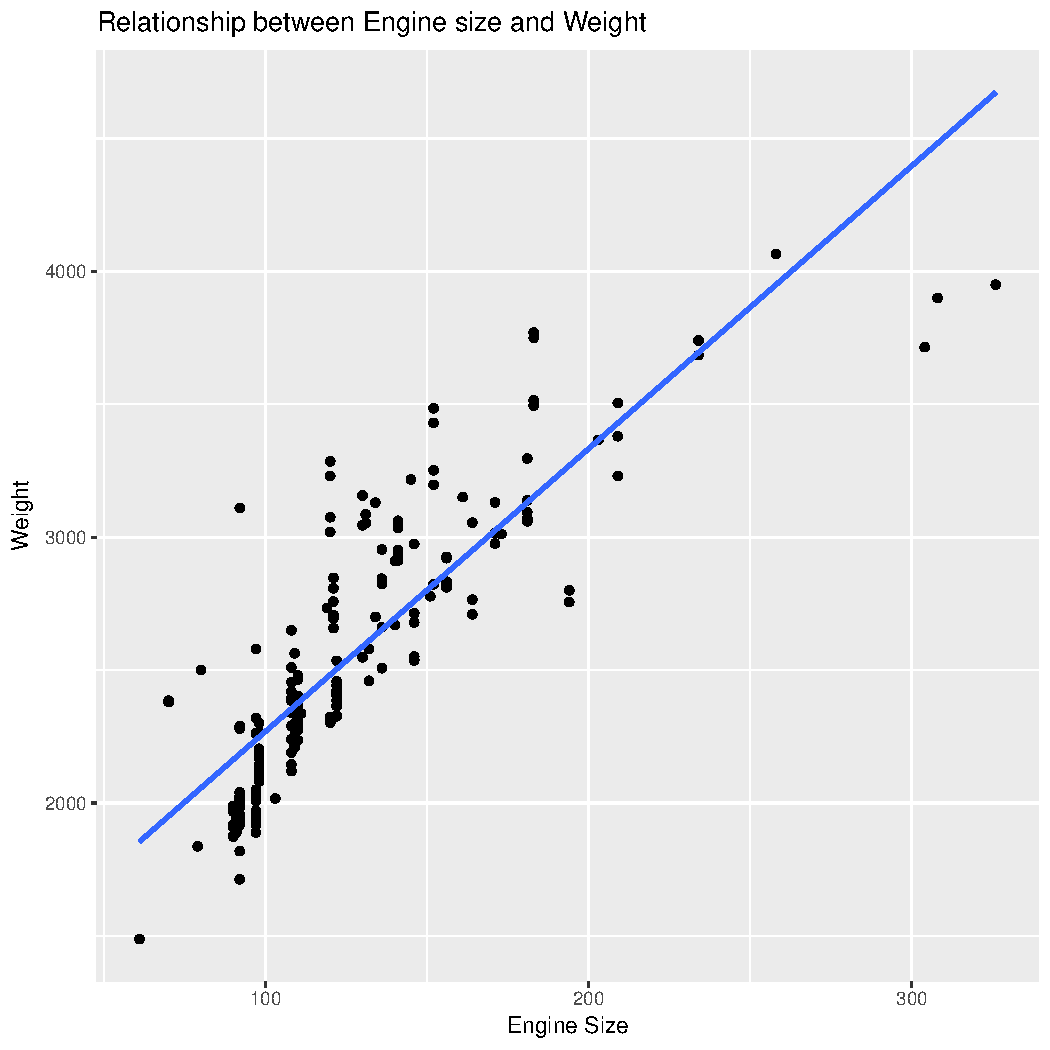
\includegraphics[width=\maxwidth]{figure/unnamed-chunk-1-1} 
\begin{kframe}\begin{alltt}
\hlkwd{ggplot}\hlstd{(imports_85,} \hlkwd{aes}\hlstd{(}\hlkwc{x} \hlstd{= Price,} \hlkwc{y} \hlstd{= Make))} \hlopt{+}
\hlkwd{geom_point}\hlstd{()} \hlopt{+}
\hlkwd{labs}\hlstd{(}\hlkwc{x} \hlstd{=} \hlstr{"Price"}\hlstd{,} \hlkwc{y} \hlstd{=} \hlstr{"Weight"}\hlstd{,}
\hlkwc{title} \hlstd{=} \hlstr{"Relationship between Price and Weight"}\hlstd{)} \hlopt{+}
\hlkwd{geom_smooth}\hlstd{(}\hlkwc{method} \hlstd{=} \hlstr{"lm"}\hlstd{,} \hlkwc{se} \hlstd{=} \hlnum{FALSE}\hlstd{)}
\end{alltt}


{\ttfamily\noindent\color{warningcolor}{\#\# Warning: Removed 4 rows containing non-finite values (stat\_smooth).}}

{\ttfamily\noindent\color{warningcolor}{\#\# Warning: Removed 4 rows containing missing values (geom\_point).}}\end{kframe}
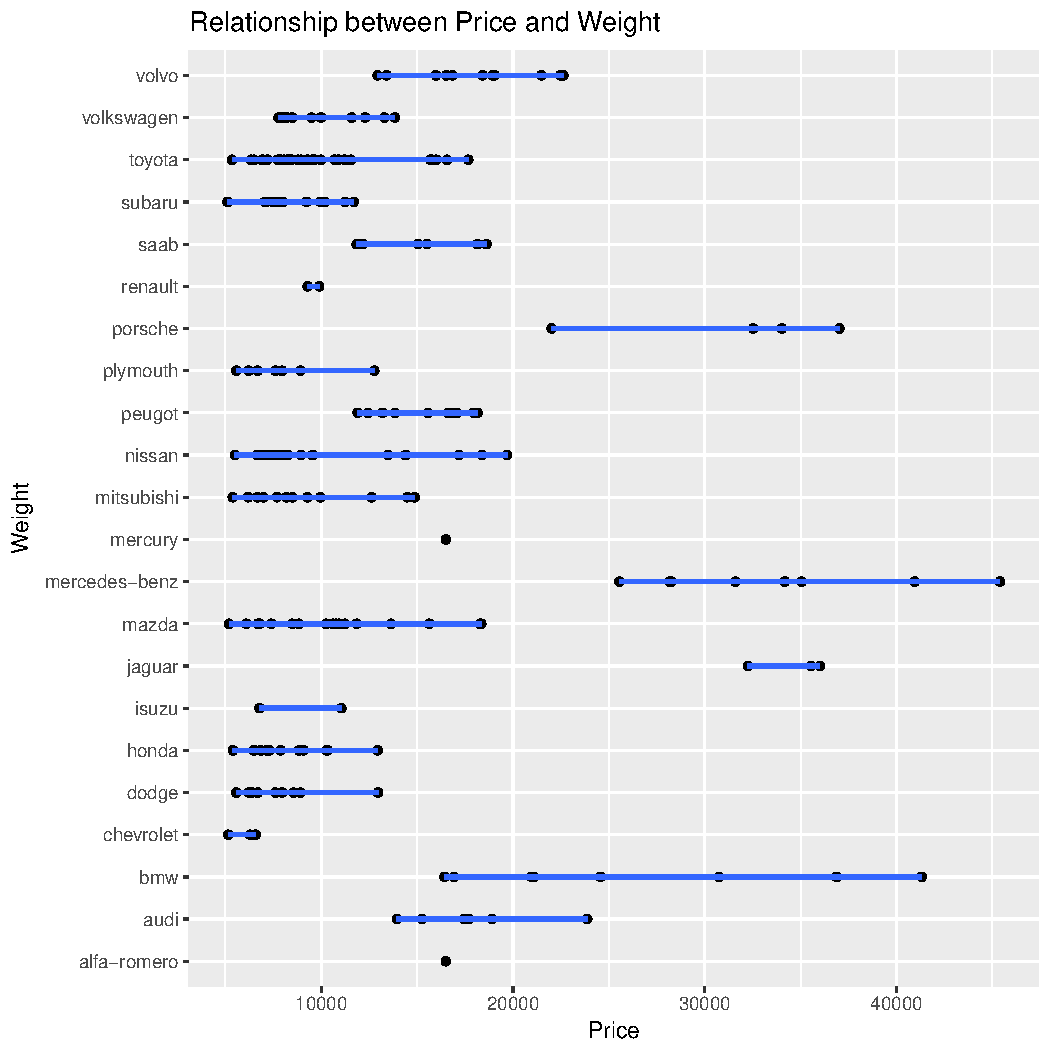
\includegraphics[width=\maxwidth]{figure/unnamed-chunk-1-2} 

\end{knitrout}

The relationship of Engine Size and Weight was a nice confirmation that my intuition works. The larger the Engine, the likelier that the Weight of the Car would be higher.


\end{document}
